% !TEX root = ../presentation.tex
% !BIB program = biber
% !TEX program = xelatex

\section{vae background and the ladder variational autoencoder (lvae)}

\begin{frame}{The Ladder Variational Autoencoder (LVAE)}
    \begin{columns}
        \begin{column}{0.5\textwidth}
            This is a Ladder VAE with three latent variables.
        \end{column}
        \begin{column}{0.5\textwidth}
            \begin{figure}[\textwidth]
            \def\col{blue}
            \tikz{
            % INFERENCE
            % nodes
            \node[obs] (x_inf) {$\xb$};%
            \node[det,above=.75cm of x_inf] (d1){$\db_1$}; %
            \node[det,above=.75cm of d1] (d2){$\db_2$}; %
            \node[det,above=.75cm of d2] (d3){$\db_3$}; %
            
            \node[latent,right=.5cm of d1] (z1_inf) {$\zb_1$}; %
            \node[latent,right=.5cm of d2] (z2_inf) {$\zb_2$}; %
            \node[latent,right=.5cm of d3] (z3_inf) {$\zb_3$}; %
            \node[above=of z3_inf, xshift=-.7cm, yshift=-1.cm] (phi) {$q_\phi(\zb|\xb)$}; 
            
            % edges
            \edge[]{x_inf}{d1}
            \edge[\col]{z2_inf}{z1_inf}
            \edge[]{d1}{d2}
            \edge[\col]{z3_inf}{z2_inf}
            \edge[]{d2}{d3}
            \edge[]{d1}{z1_inf}
            \edge[]{d2}{z2_inf}
            \edge[]{d3}{z3_inf}
        
            % GENERATIVE
            % nodes
            \node[latent,right=.75cm of z3_inf] (z3_gen) {$\zb_3$}; %
            \node[latent,right=.75cm of z2_inf] (z2_gen) {$\zb_2$}; %
            \node[latent,right=.75cm of z1_inf] (z1_gen) {$\zb_1$}; %
            \node[obs,below=.75cm of z1_gen] (x_gen) {$\xb$};
            \node[above=of z3_gen, yshift=-1.cm] (theta) {$p_\thetab(\xb,\zb)$}; 
        
            
            % edges
            \edge[\col]{z3_gen}{z2_gen}
            \edge[\col]{z2_gen}{z1_gen}
            \edge[]{z1_gen}{x_gen}
            
            }
            \end{figure}
        \end{column}
    \end{columns}
\end{frame}


\begin{frame}{Overview}
    Understanding the Ladder VAE is not so much about understanding the specific architecture as it is about:
    \begin{itemize}
        \item[a)] understanding the reason for choosing it,
        \item[b)] which other options were available,
        \item[c)] and why they don't work as well.
    \end{itemize} 
\end{frame}


\begin{frame}{A generative model from latent variables}
    \begin{columns}[c]
        \begin{column}{.7\textwidth}
            Suppose data $\xb \sim p (\xb)$ is generated via some underlying \textit{latent} variable $\zb$. Then
            \begin{equation}
                p(\xb) = \int p(\xb,\zb) \text{d}\zb = \int p(\xb|\zb)p(\zb) \text{d}\zb.
            \end{equation}
            We would like to 
            \begin{itemize}
                \item[a)] \textit{infer} the latent variables $\zb$ given $\xb$
                \item[b)] \textit{generate} the observed variable $\xb$ given $\zb$
            \end{itemize}
        \end{column}
        \begin{column}{.3\textwidth}
            \begin{figure}[\textwidth]
                \tikz{
                    % GENERATIVE
                    % nodes$
                    \node[obs] (x_gen) {$\xb$};%
                    \node[latent,above=.75cm of x_gen](z1_gen){$\zb$}; %
                    \node[above=of z1_gen, yshift=-1.cm] (phi) {$p(\xb,\zb)$}; 

                    % edges
                    \edge[]{z1_gen}{x_gen};
                }
            \end{figure}
        \end{column}
    \end{columns}
\end{frame}


\begin{frame}{Exact inference}
    \begin{columns}
        \begin{column}{0.7\textwidth}
            We can choose some simple model for $p(\xb,\zb)$ (denoted $p_\thetab$ and parameterized by $\thetab$).
            \vspace{3mm}
            
            Bayes theorem then gives us the true model posterior,
            \begin{equation}
                p_\thetab(\zb|\xb) = \frac{p_\thetab(\xb,\zb)}{p_\thetab(\xb)} = \frac{p_\thetab(\xb|\zb)p_\thetab(\zb)}{\int p_\thetab(\xb|\zb)p_\thetab(\zb) \text{d}\zb}.
            \end{equation}
            But this only works if we can integrate over the latent variable $\zb$ and the model $p_\thetab(\xb|\zb)$.
        \end{column}
        \begin{column}{.3\textwidth}
            \begin{figure}[\textwidth]
                \tikz{
                    % GENERATIVE
                    % nodes$
                    \node[obs] (x_gen) {$\xb$};%
                    \node[latent,above=.75cm of x_gen](z1_gen){$\zb$}; %
                    \node[above=of z1_gen, yshift=-1.cm] (phi) {$p(\xb,\zb)$}; 
            
                    % edges
                    \edge[]{z1_gen}{x_gen};
                }
            \end{figure}
        \end{column}
    \end{columns}
\end{frame}


\begin{frame}{Exact inference becomes intractable}
    Suppose we want to model complex data where $\vert\xb\vert = D \gg 1$, such as images, audio or graphs.
    \vspace{3mm}

    We might choose to parameterize $p(\xb,\zb)$ with a neural network model with parameters $\thetab$ and try to \textit{learn} $p_\thetab(\xb) \approx p(\xb)$.

    \begin{equation}
        p_\thetab(\xb, \zb) = p_\thetab(\xb|\zb)p(\zb)
    \end{equation}
    
    where we could choose $p(\zb)=\mathcal{N}(\0,\1)$.
    \vspace{3mm}

    However, this comes at the cost of making integrals over the latent variables intractable and hence, \textbf{we can no longer directly compute} $p_\thetab(\xb)$.
\end{frame}


\begin{frame}{Variational inference and the ELBO}
    Introduce some \textit{variational} distribution $q_\phi(\zb|\xb)$ (parameterized by $\phi$)
    \begin{align}
        \log p(\xb) &= \log \int p_\thetab(\xb,\zb) \,\text{d}\zb \notag \\
                    &= \log \int q_\phi(\zb|\xb) \frac{p_\thetab(\xb,\zb)}{q_\phi(\zb|\xb)} \,\text{d}\zb \notag \\
                    &\geq \int q_\phi(\zb|\xb) \log \frac{p_\thetab(\xb,\zb)}{q_\phi(\zb|\xb)} \,\text{d}\zb \notag \\
                    &= \mathbb{E}_{q_\phi(\zb|\xb)} \left[ \log \frac{p_\thetab(\xb,\zb)}{q_\phi(\zb|\xb)} \right] \notag \\
                    &= \mathbb{E}_{q_\phi(\zb|\xb)} \left[ \log p_\thetab(\xb|\zb) + \log p_\thetab(\zb) - \log q_\phi(\zb|\xb) \right] \notag\\
                    &\equiv \underbrace{\mathcal{L}(\xb;\thetab,\phi)}_{\text{evidence lower bound}}
    \end{align}
\end{frame}


\begin{frame}{The variational autoencoder (VAE)}
    \begin{columns}
        \begin{column}{0.8\textwidth}
        Suppose we parameterize $q_\phi(\zb|\xb)$ by a model with parameters $\phi$.
        Then we can optimize both $\{\thetab,\phi\}$ jointly by maximizing the ELBO.

        \begin{equation}
            \{\thetab^{*},\phi^{*}\} = \underset{\{\thetab, \phi\}}{\arg\max} \, \mathcal{L}(\xb;\thetab,\phi)
        \end{equation}
        
        The result is the VAE \cite{kingma_autoencoding_2014} consisting of
        \begin{itemize}
            \item[a)] an \textit{inference model} (or \textit{encoder}) $q\phi(\zb|\xb)$ which approximates the intractable true posterior $p(\zb|\xb)$.
            \item[b)] a \textit{generative model} (or \textit{decoder}) $p_\thetab(\xb|\zb)$ which can generate new samples from the prior $p(\zb)$, or "reconstruct" with proposals from $q_\phi(\zb|\xb)$.
        \end{itemize}
        
        \end{column}

        \begin{column}{0.2\textwidth}
            \begin{figure}[.5\textwidth]
            \tikz{
                % inference
                % nodes
                \node[obs] (x_inf) {$\xb$};%
                \node[latent,above=.75cm of x_inf](z1_inf){$\zb$}; %
                \node[above=of z1_inf, yshift=-1.cm] (phi) {$q_\phi(\zb|\xb)$}; 
                
                % edges
                \edge[]{x_inf}{z1_inf};
                
                % generative
                % nodes$
                \node[obs,right=0.75cm of x_inf] (x_gen) {$\xb$};%
                \node[latent,above=.75cm of x_gen](z1_gen){$\zb$}; %
                \node[above=of z1_gen, yshift=-1.cm] (theta) {$p_\thetab(\xb,\zb)$}; 
                
                % edges
                \edge[]{z1_gen}{x_gen};
            }
            \end{figure}
        
        \end{column}
    \end{columns}
\end{frame}


\begin{frame}{Limitations of VAEs}
    \begin{columns}
        \begin{column}{0.8\textwidth}
            The VAE uses a mean field approximation for most common variational posteriors.
            \begin{equation}
                q(\zb) = \prod_{i} q(z_i)
            \end{equation}
            \begin{itemize}
                \item Assumes independence between latent variables.
                \item Model cannot learn covariance between latents.
                \item This limits expressivity as we cannot expect to always match the true posterior well.
            \end{itemize}
            {\small \textit{E.g. a vehicle's color is often dependent on its type (fire truck, police car, bus, taxi etc.) but these are coded independently in $\zb$}.}
        \end{column}
        \begin{column}{0.2\textwidth}
            \begin{figure}[.5\textwidth]
            \tikz{
                % inference
                % nodes
                \node[obs] (x_inf) {$\xb$};%
                \node[latent,above=.75cm of x_inf](z1_inf){$\zb$}; %
                \node[above=of z1_inf, yshift=-1.cm] (phi) {$q_\phi(\zb|\xb)$}; 
                
                % edges
                \edge[]{x_inf}{z1_inf};
                
                % generative
                % nodes$
                \node[obs,right=0.75cm of x_inf] (x_gen) {$\xb$};%
                \node[latent,above=.75cm of x_gen](z1_gen){$\zb$}; %
                \node[above=of z1_gen, yshift=-1.cm] (theta) {$p_\thetab(\xb,\zb)$}; 
                
                % edges
                \edge[]{z1_gen}{x_gen};
            }
            \end{figure}
        \end{column}
    \end{columns}
\end{frame}


\begin{frame}{Hierarchical VAE}
    \begin{columns}
        \begin{column}{0.8\textwidth}
            To avoid these limitations, we can introduce a hierarchy of additional latent variables $\zb=\zb_1,\dots,\zb_L$. For $L=3$,
            \begin{equation}
                p_\thetab(\xb|\zb) = p_\thetab(\xb|\zb_1) p_\thetab(\zb_1|\zb_2) p(\zb_3).
            \end{equation}
            We can straightforwardly generalize the inference model,
            \begin{equation}
                q_\phi(\zb|\xb) = q_\phi(\zb_1|\xb)q_\phi(\zb_2|\zb_1)q_\phi(\zb_3|\zb_2).
            \end{equation}
            This is called \textit{bottom-up} inference.
        \end{column}
        \begin{column}{0.2\textwidth}
            \begin{figure}[.5\textwidth]
                \tikz{
                    % INFERENCE
                    % nodes
                    \node[obs] (x_inf) {$\xb$};%
                    \node[latent,above=.75cm of x_inf](z1_inf){$\zb_1$}; %
                    \node[latent,above=.75cm of z1_inf](z2_inf){$\zb_2$}; %
                    \node[latent,above=.75cm of z2_inf](z3_inf){$\zb_3$}; %
                    \node[above=of z3_inf, yshift=-1.cm] (phi) {$q_\phi(\zb|\xb)$}; 
                    
                    % edges
                    \edge[]{x_inf}{z1_inf};
                    \edge[]{z1_inf}{z2_inf};
                    \edge[]{z2_inf}{z3_inf};
                    
                    % GENERATIVE
                    % nodes
                    \node[obs,right=0.75cm of x_inf] (x_gen) {$\xb$};%
                    \node[latent,above=.75cm of x_gen](z1_gen){$\zb_1$}; %
                    \node[latent,above=.75cm of z1_gen](z2_gen){$\zb_2$}; %
                    \node[latent,above=.75cm of z2_gen](z3_gen){$\zb_3$}; %
                    \node[above=of z3_gen, yshift=-1.cm] (phi) {$p_\thetab(\xb,\zb)$}; 
                    
                    % edges
                    \edge[]{z3_gen}{z2_gen};
                    \edge[]{z2_gen}{z1_gen};
                    \edge[]{z1_gen}{x_gen};
                }
            \end{figure}
        \end{column}
    \end{columns}
\end{frame}


\begin{frame}{Challenges of hierarchical VAEs}
    Consider a simple model $p_{\text{simple}}(\xb)$ without any latent variables. We can rewrite the likelihood as,
    \begin{align*}
        \mathbb{E}_{p(\xb)} \left[ \log p_{\text{simple}}(\xb) \right] &= \mathbb{E}_{p(\xb)} \left[ \log \left( p(\xb) \frac{p_{\text{simple}}(\xb)}{p(\xb)} \right) \right] \\
                                                                    %  &= -\mathcal{H}(p) - D_\text{KL} \left( p(\xb) || p_\text{simple}(\xb) \right)
                                                                    &= -\underbrace{\mathcal{H}(p)}_{\text{data entropy}} - \underbrace{D_\text{KL} \left( p(\xb) || p_\text{simple}(\xb) \right)}_{\text{divergence from data distribution}}
    \end{align*}
    where $\mathcal{H}(p)=\mathbb{E}_{p(\xb)}[\log p(\xb)]$.
\end{frame}


\begin{frame}{Challenges of hierarchical VAEs}
    \begin{columns}
        \begin{column}{1\textwidth}
            Let's do the same for a VAE $p_\thetab(\xb)$ with ELBO given by
            \begin{equation}
                \log p_\thetab(\xb) \geq \mathbb{E}_{q_\phi(\zb|\xb)} \left[ \log \frac{p_\thetab(\xb|\zb)p_\thetab(\zb)}{q_\phi(\zb|\xb)} \right].
            \end{equation}
            The expectation over the data becomes,
            \begin{align}
                \mathbb{E}_{p(\xb)} \left[ \log p_\thetab(\xb) \right] \geq& \mathbb{E}_{p(\xb)} \left[ \log \left( p(\xb) \frac{p_\thetab(\xb)}{p(\xb)} \right) \right] \notag \\
                                                                    =& -\mathcal{H}(p) - D_\text{KL} \left( p(\xb) || p_\thetab(\xb) \right) \notag \\
                                                                        & \quad - \underbrace{\mathbb{E}_{p(\xb)} \left[ D_\text{KL}\left( q_\phi(\zb|\xb) || p_\thetab(\zb|\xb) \right) \right]}_{\text{divergence from true posterior}}
            \end{align}
            Compared to the simple model, we incur an \textbf{additional cost} for the latent variable given by the divergence from the true model posterior.
        \end{column}
    \end{columns}
\end{frame}


\begin{frame}{Challenges of hierarchical VAEs}
    For a hierarchical VAE with two latent variables
    \begin{align}
        \mathbb{E}_{p(\xb)} \left[ \log p_\thetab(\xb) \right] \geq& \mathbb{E}_{p(\xb)} \left[ \log \left( p(\xb) \frac{p_\thetab(\xb)}{p(\xb)} \right) \right] \notag \\
                                                            =& -\mathcal{H}(p) - D_\text{KL} \left( p(\xb) || p_\thetab(\xb) \right) \notag \\
                                                                & \quad - \mathbb{E}_{p(\xb)} \mathbb{E}_{q_\phi(\zb_1|\xb)} \left[ D_\text{KL}\left( q_\phi(\zb_2|\zb_1) || p_\thetab(\zb_2|\zb_1) \right) \right] \notag \\
                                                                & \quad - \mathbb{E}_{p(\xb)} \left[ D_\text{KL}\left( q_\phi(\zb_1|\xb) || p_\thetab(\zb_1|\xb) \right) \right]
    \end{align}

    The cost is \textbf{incurred for each additional latent} we add to the hierarchy.
    \vspace{3mm}
    
    Hence, each latent will only be used by the model if we get an \textbf{opposite equal or larger improvement} in the ELBO.
\end{frame}


\begin{frame}{{\tiny (Failing to)} Dodge the challenges}
    \begin{columns}
        \begin{column}{0.77\textwidth}
            There's a few common ways to try and dodge these issues:
            \begin{itemize}
                \item Skip connections \cite{dieng_avoiding_2019, maaloe_biva_2019}
                \item Free bits in the KL-terms \cite{kingma_improved_2016}
                \item Deterministic warmup \cite{sonderby_ladder_2016}
                \item Batch normalization/weight normalization \cite{ioffe_batch_2015, salimans_weight_2016}
            \end{itemize}

            \vspace{5mm}
            None of them work for more than around 5 latent variables.
        \end{column}
        \begin{column}{0.3\textwidth}
            \begin{figure}[.5\textwidth]
                \tikz{
                    % INFERENCE
                    % nodes
                    \node[obs] (x_inf) {$\xb$};%
                    \node[latent,above=.75cm of x_inf](z1_inf){$\zb_1$}; %
                    \node[latent,above=.75cm of z1_inf](z2_inf){$\zb_2$}; %
                    \node[latent,above=.75cm of z2_inf](z3_inf){$\zb_3$}; %
                    \node[above=of z3_inf, yshift=-1.cm] (phi) {$q_\phi(\zb|\xb)$}; 
                    
                    % edges
                    \edge[]{x_inf}{z1_inf};
                    \edge[]{z1_inf}{z2_inf};
                    \edge[]{z2_inf}{z3_inf};
                    \edge[dashed, bend left]{x_inf}{z2_inf};
                    \edge[dashed, bend left]{x_inf}{z3_inf};
                    
                    % GENERATIVE
                    % nodes
                    \node[obs,right=0.75cm of x_inf] (x_gen) {$\xb$};%
                    \node[latent,above=.75cm of x_gen](z1_gen){$\zb_1$}; %
                    \node[latent,above=.75cm of z1_gen](z2_gen){$\zb_2$}; %
                    \node[latent,above=.75cm of z2_gen](z3_gen){$\zb_3$}; %
                    \node[above=of z3_gen, yshift=-1.cm] (phi) {$p_\thetab(\xb,\zb)$}; 
                    
                    % edges
                    \edge[]{z3_gen}{z2_gen};
                    \edge[]{z2_gen}{z1_gen};
                    \edge[]{z1_gen}{x_gen};
                    \edge[dashed, bend left]{z2_gen}{x_gen};
                    \edge[dashed, bend left]{z3_gen}{x_gen};
                }
            \end{figure}
        \end{column}
    \end{columns}
\end{frame}



\begin{frame}{The Ladder VAE}
    \begin{columns}
        \begin{column}{0.6\textwidth}
            The LVAE introduces a \textit{top-down} inference path,
            \begin{equation}
                q_\phi(\zb|\xb) = q_\phi(\zb_L|\xb) \prod_{i=1}^{L-1} q_\phi(\zb_{i}|\zb_{i+1}).
            \end{equation}
            It is aided by a \textbf{deterministic bottom-up path} and \textbf{{\color{blue} parameter sharing}} between the inference and generative models.
        \end{column}
        \begin{column}{0.4\textwidth}
            \begin{figure}[\textwidth]
            \def\col{blue}
            \tikz{
                % INFERENCE
                % nodes
                \node[obs] (x_inf) {$\xb$};%
                \node[det,above=.75cm of x_inf] (d1){$\db_1$}; %
                \node[det,above=.75cm of d1] (d2){$\db_2$}; %
                \node[det,above=.75cm of d2] (d3){$\db_3$}; %
                
                \node[latent,right=.5cm of d1] (z1_inf) {$\zb_1$}; %
                \node[latent,right=.5cm of d2] (z2_inf) {$\zb_2$}; %
                \node[latent,right=.5cm of d3] (z3_inf) {$\zb_3$}; %
                \node[above=of z3_inf, xshift=-.7cm, yshift=-1.cm] (phi) {$q_\phi(\zb|\xb)$}; 
                
                % edges
                \edge[]{x_inf}{d1}
                \edge[\col]{z2_inf}{z1_inf}
                \edge[]{d1}{d2}
                \edge[\col]{z3_inf}{z2_inf}
                \edge[]{d2}{d3}
                \edge[]{d1}{z1_inf}
                \edge[]{d2}{z2_inf}
                \edge[]{d3}{z3_inf}

                % GENERATIVE
                % nodes
                \node[latent,right=.75cm of z3_inf] (z3_gen) {$\zb_3$}; %
                \node[latent,right=.75cm of z2_inf] (z2_gen) {$\zb_2$}; %
                \node[latent,right=.75cm of z1_inf] (z1_gen) {$\zb_1$}; %
                \node[obs,below=.75cm of z1_gen] (x_gen) {$\xb$};
                \node[above=of z3_gen, yshift=-1.cm] (theta) {$p_\thetab(\xb,\zb)$}; 
                
                % edges
                \edge[\col]{z3_gen}{z2_gen}
                \edge[\col]{z2_gen}{z1_gen}
                \edge[]{z1_gen}{x_gen}
            }
            \end{figure}
        \end{column}
    \end{columns}
\end{frame}


\begin{frame}{Benchmarks}
    \begin{table}[]
        \centering
        \begin{tabular}{lr}
        \toprule
        Model & $\geq \log p(\xb)$ \\
        \midrule
        VAE + NF ($L=1$) & -85.10 \\
        IWAE ($L=2$, $K=1$) & -85.33 \\
        IWAE ($L=2$, $K=50$) & -82.90 \\
        VAE + VGP ($L=2$) & -81.90 \\
        \midrule
        LVAE ($L=5$) & -82.12 \\
        LVAE + finetuning ($L=5$) & -81.84 \\
        LVAE + finetuning ($L=5$, $K=10$) & -81.74 \\
        \bottomrule
        \end{tabular}
        \caption{Results on dynamically binarized MNIST.}
    \end{table}
\end{frame}


\begin{frame}{Latent space activation}
    \begin{figure}[\textwidth]
        \centering
        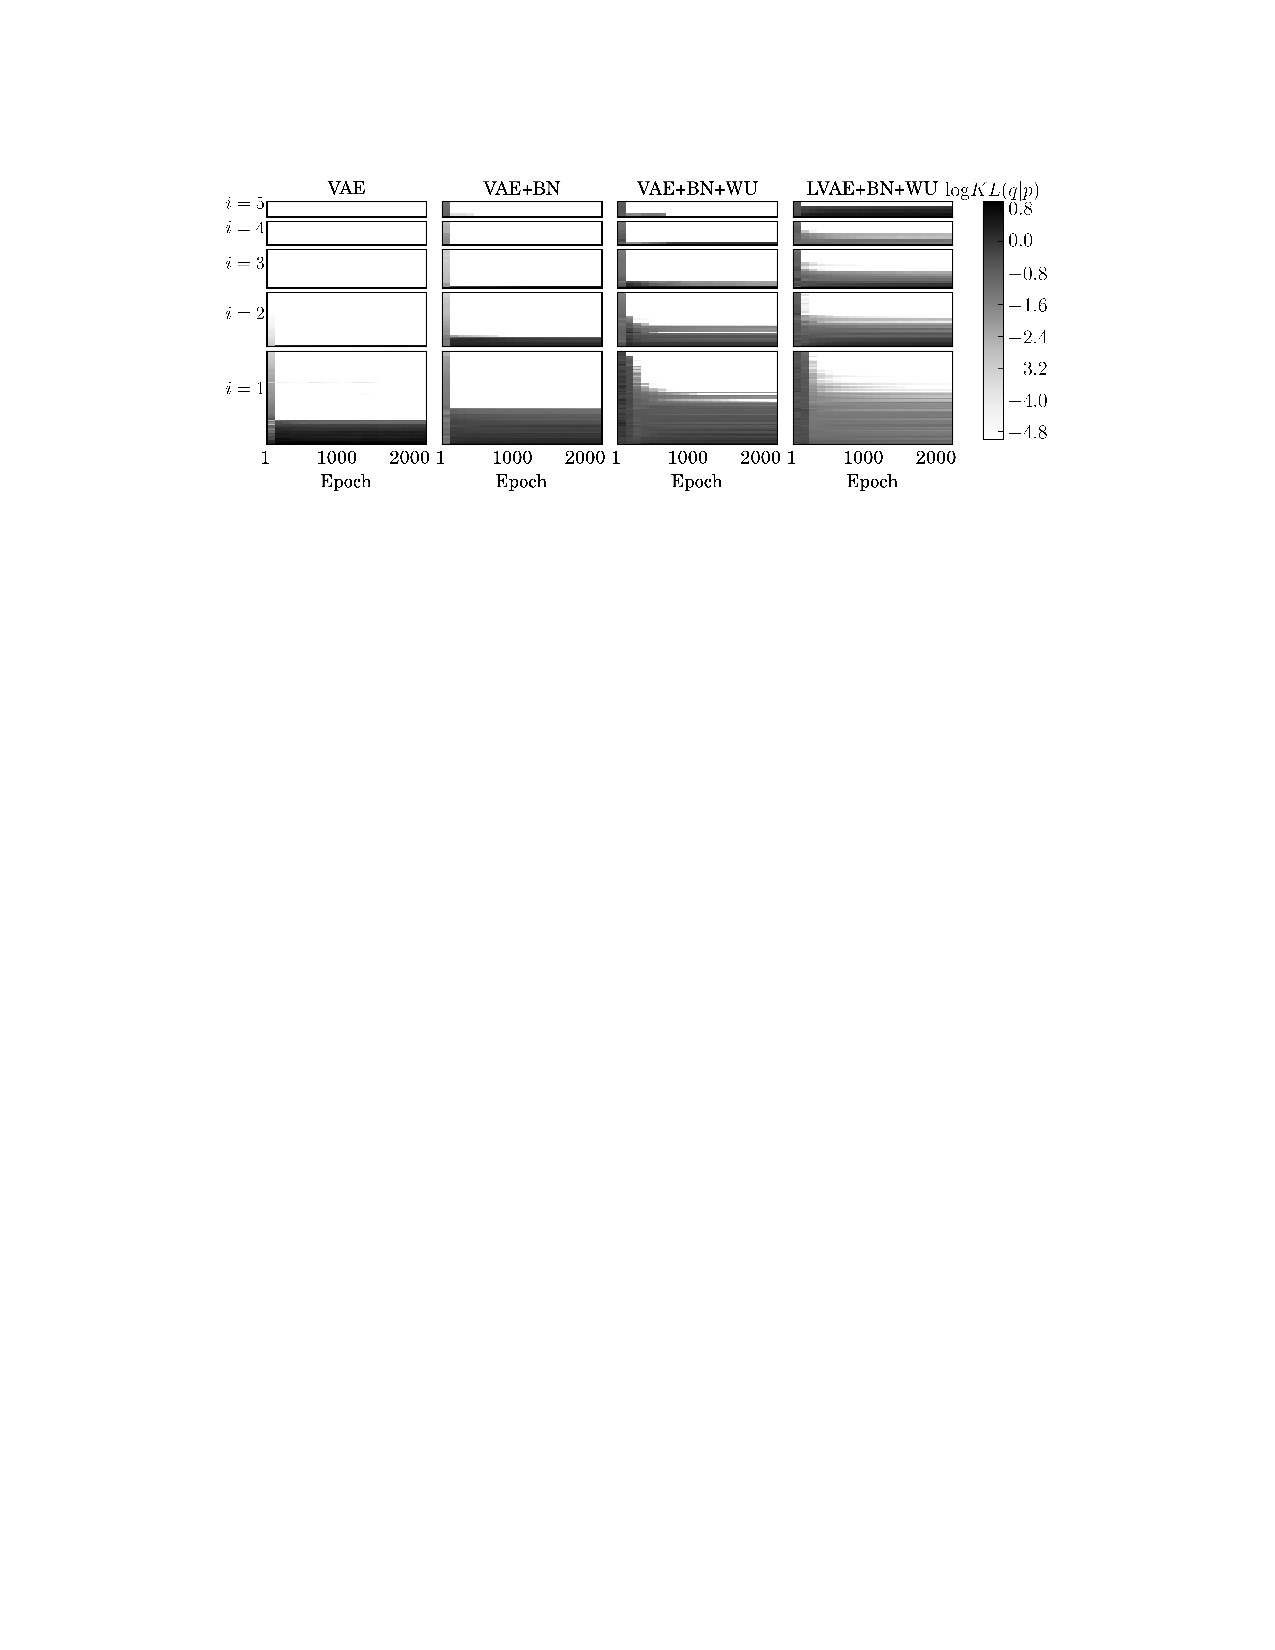
\includegraphics[scale=0.85]{figures/ladder_vae_latent_activations.pdf}
        \caption{Element-wise KL-divergences in each latent variable $q(\zb_i|\zb_{i-1})$ with $\zb_0\equiv \xb$.}
    \end{figure}
\end{frame}


\begin{frame}{Latent space representation}
    \begin{figure}[\textwidth]
        \centering
        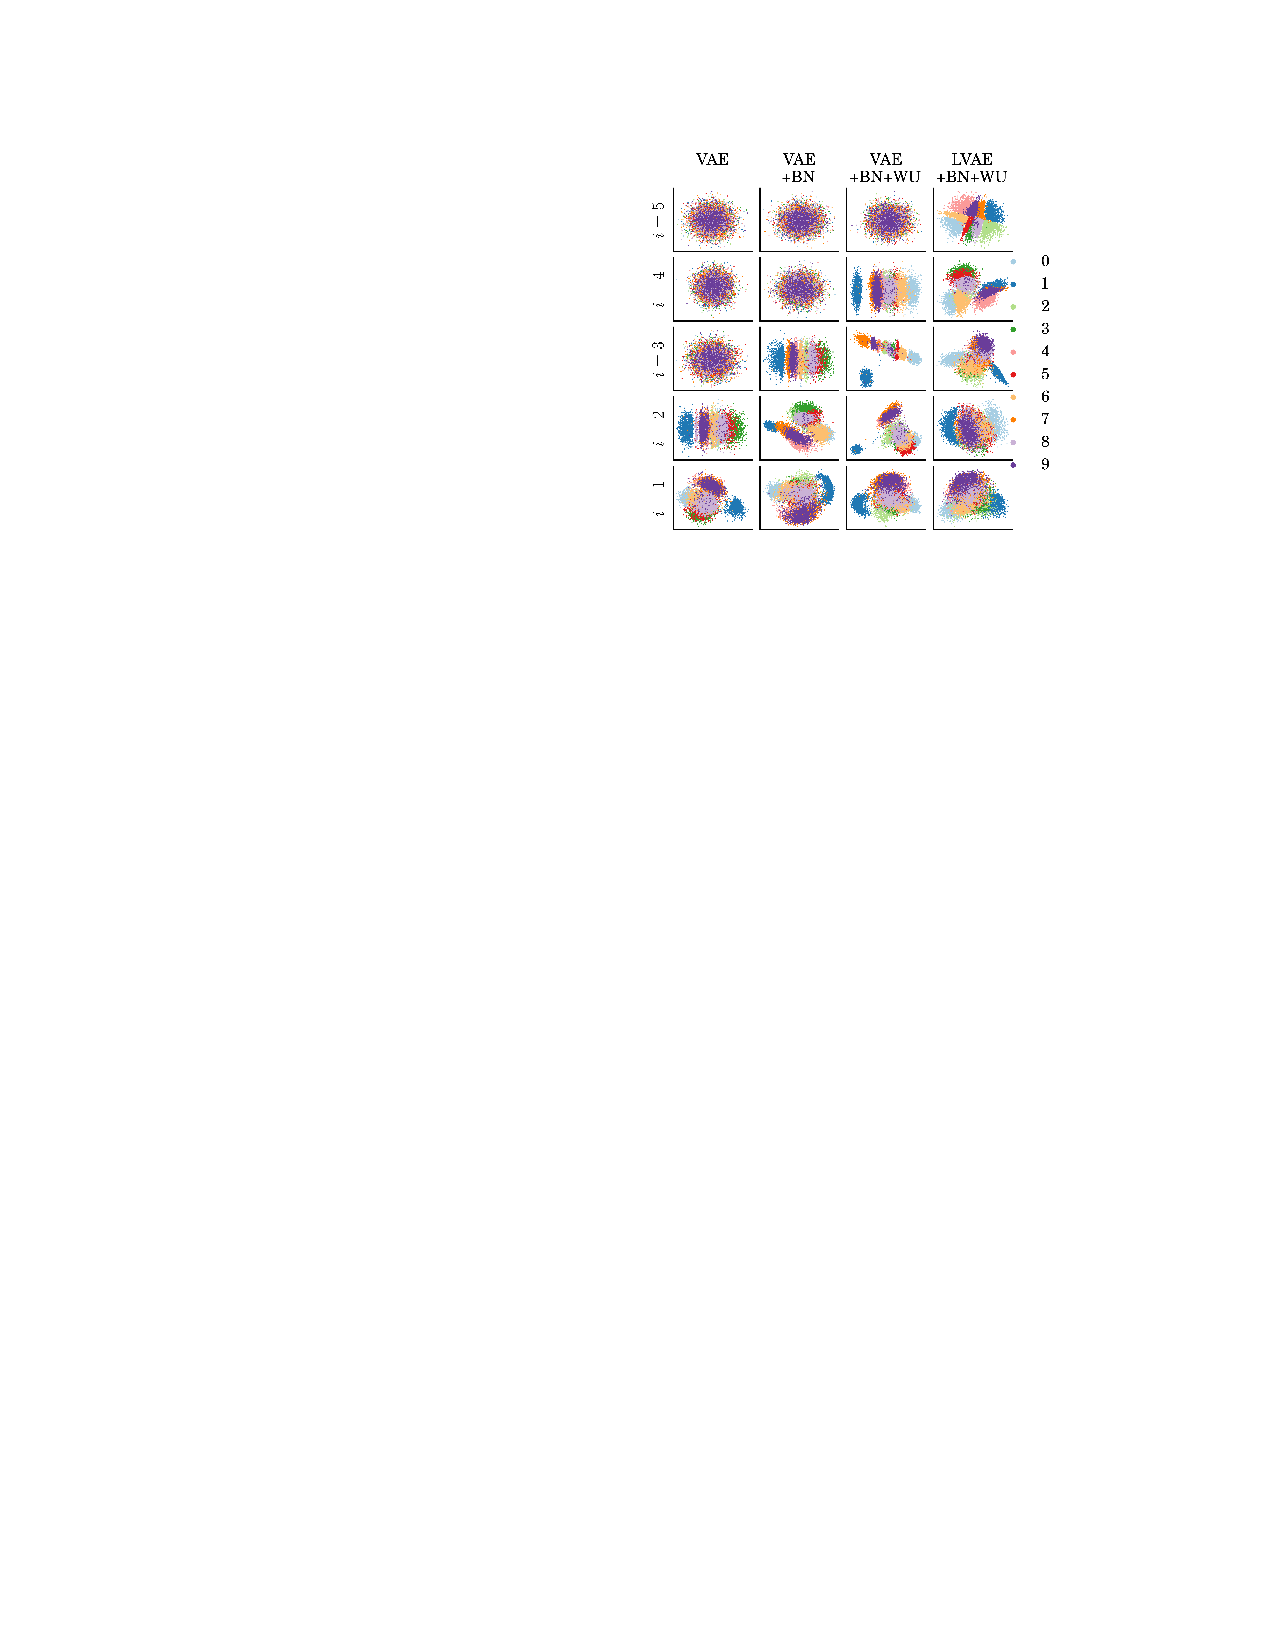
\includegraphics[scale=1]{figures/ladder_vae_pca.pdf}
        \caption{PCA of latent samples from $q(\zb_i|\zb_{i-1})$ with $\zb_0\equiv \xb$.}
    \end{figure}
\end{frame}


\begin{frame}{Recent work}
    \begin{figure}[\textwidth]
        \centering
        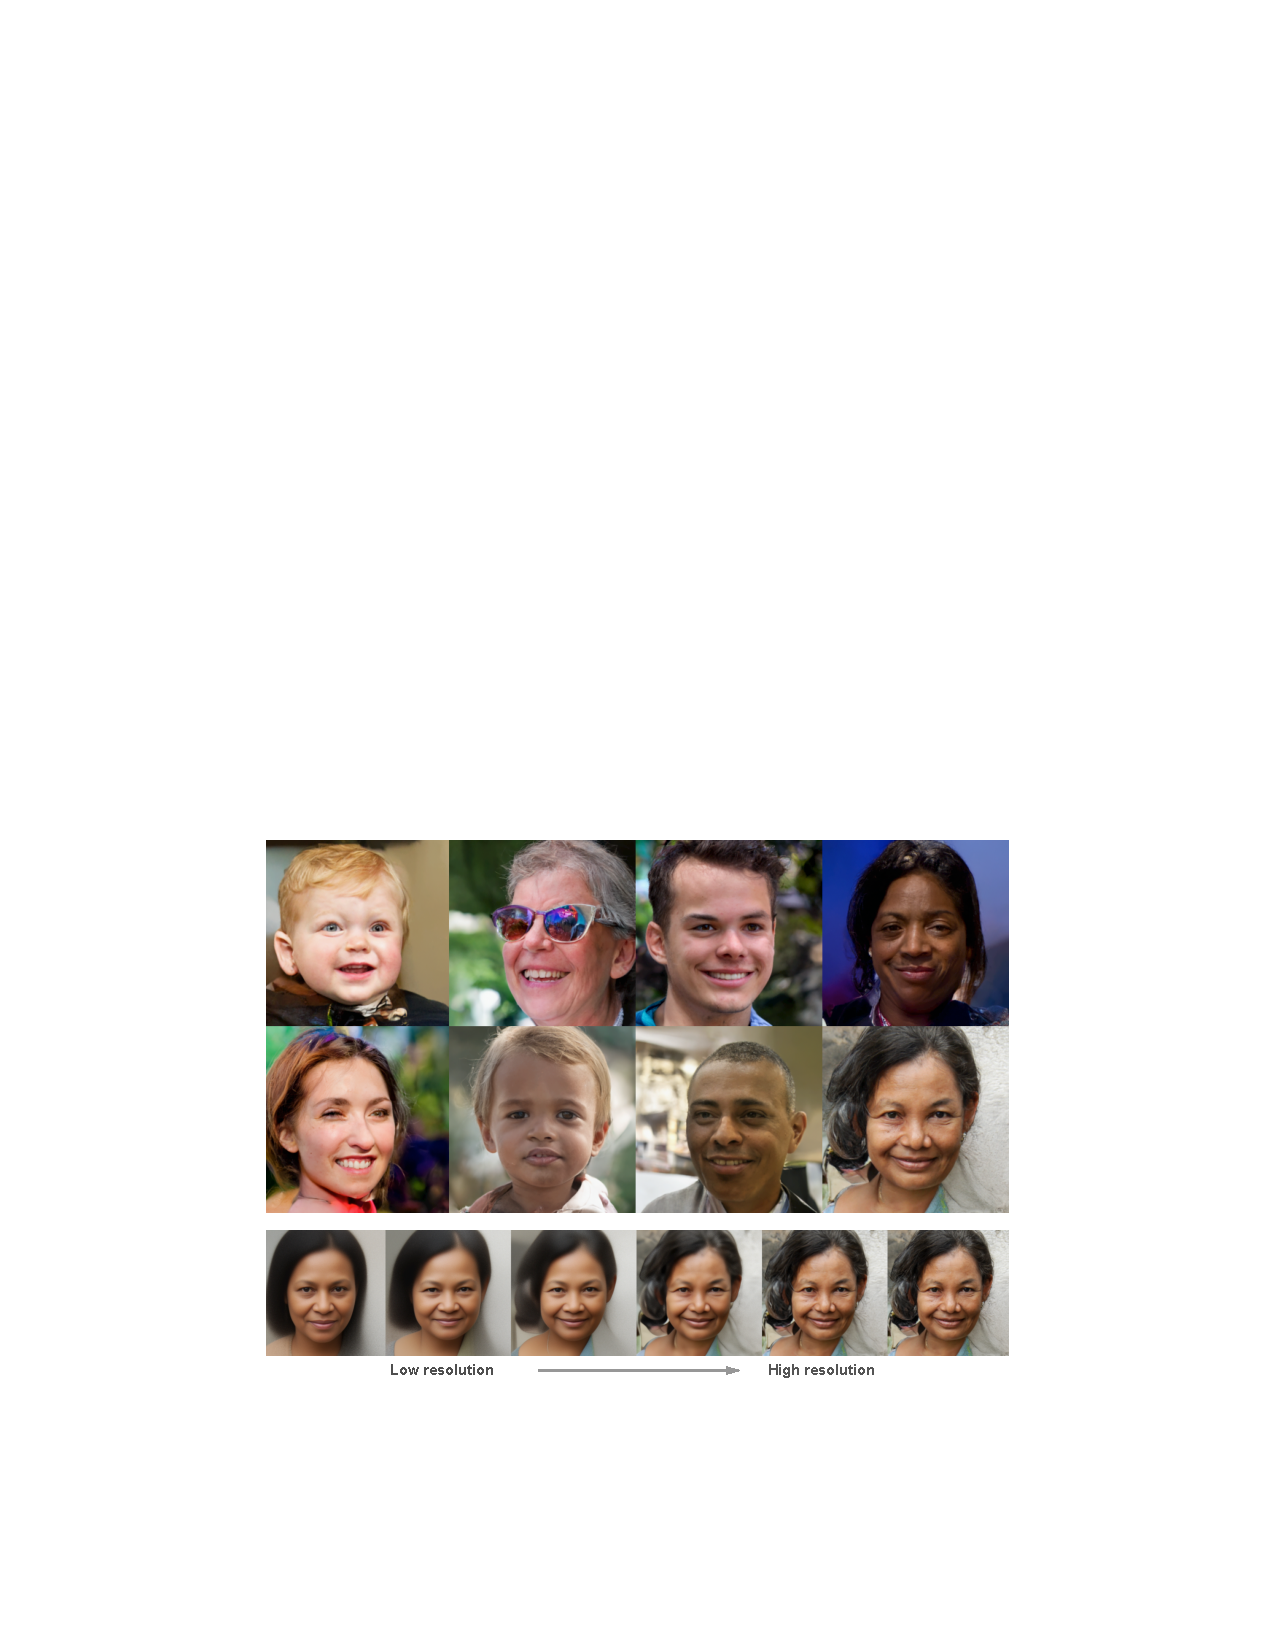
\includegraphics[scale=0.7]{figures/child_faces.pdf}
        \caption{Samples from the generative model of \cite{child_very_2021} with more than 70 latents.}
    \end{figure}
\end{frame}
